\documentclass[sigconf]{acmart}
\usepackage[utf8]{inputenc}

\settopmatter{printacmref=false}
\renewcommand\footnotetextcopyrightpermission[1]{} % removes footnote with conference information in first column
\pagestyle{plain}

\usepackage{url}
\usepackage{hyperref}
\hypersetup{
    colorlinks=true,
    linkcolor=blue,
    filecolor=magenta,      
    urlcolor=cyan,
}
\urlstyle{same}


\usepackage{listings}

% Enabling Javascript syntax highlight in code snippet - BEGIN 
% https://tex.stackexchange.com/questions/89574/language-option-supported-in-listings
\usepackage{color}
\definecolor{lightgray}{rgb}{.9,.9,.9}
\definecolor{darkgray}{rgb}{.4,.4,.4}
\definecolor{purple}{rgb}{0.65, 0.12, 0.82}
\definecolor{darkgreen}{rgb}{0, .64, 0}

\lstdefinelanguage{JavaScript}{
  keywords={typeof, new, true, false, catch, function, return, null, catch, switch, var, if, in, while, do, else, case, break},
  keywordstyle=\color{blue}\bfseries,
  ndkeywords={class, export, boolean, throw, implements, import, this},
  ndkeywordstyle=\color{darkgray}\bfseries,
  identifierstyle=\color{black},
  sensitive=false,
  comment=[l]{//},
  morecomment=[s]{/*}{*/},
  commentstyle=\color{purple}\ttfamily,
  stringstyle=\color{darkgreen}\ttfamily,
  morestring=[b]',
  morestring=[b]"
}

\lstset{
   language=JavaScript,
   extendedchars=true,
   basicstyle=\footnotesize\ttfamily,
   showstringspaces=false,
   showspaces=false,
   numbers=left,
   numberstyle=\footnotesize,
   numbersep=9pt,
   tabsize=2,
   breaklines=true,
   showtabs=false,
   captionpos=b
}
% Enabling Javascript syntax highlight in code snippet - END

\newcommand{\APIName}{Successorships}

\newcommand{\APIshort}{ships}

%opening
\title{Who is the next server? Enabling fault-tolerant local Webapps}

\author{Arthur Marques \qquad Felix Grund \qquad Paul Cernek}
\affiliation{
    \institution{University of British Columbia}
    \city{Vancouver} 
    \state{BC} 
  }

\begin{document}

\maketitle

\begin{abstract}
As networking capabilities become more ubiquitous across different types of devices, applications that communicate over local area networks are becoming increasingly common.
This trend has been accelerated by the adoption of zero-configuration (zeroconf) networking standards that eliminate the burden of setup procedures.
Applications operating in zeroconf settings often face the challenge of maintaining reliability and consistency in the face of wireless links and mobile devices, resulting in potentially intermittent connectivity between hosts.
Fault-tolerance is thus a desirable property for such applications, but it can be difficult to achieve in practice.
To this end, we introduce Successorships, a JavaScript library that provides the appealing qualities of zeroconf enriched with fault-tolerance, to applications running in the browser.
Our library enables graceful recovery after server failure by handing over the server role to one of the clients currently in the network.
We evaluate our approach with a sample application, focusing on usage scenarios that involve interactions between users walking in and out of a single room. 
We find that our library recovers from failures gracefully after an average of 3.5 seconds, and that application state is maintained with eventual consistency.
\end{abstract}

\section{Introduction}
\label{sec:introduction}

Throughout the last decade we have seen the Internet become the most commonly used infrastructure for communication. Regardless of physical location, people and their devices communicate via messengers and VoIP, and collaborate via live editing tools such as Google Docs, Sheets, and, Slides. 
At the same time, we have seen the paradigm of applications communicating over local area networks become increasingly common for certain scenarios like home entertainment (e.g. Google Chromecast, Apple Bonjour, Spotify Connect) or Wi-Fi printers. 
With the advancements of ``smart'' devices and the ``Internet of Things'' (IoT) it is likely that this trend will grow beyond these currently still narrowly scoped application domains.

The adoption of standards that eliminate the burden of manual configuration of network devices further contributes to this movement. One such standard that has received widespread usage is Zero-configuration networking~\cite{guttman_2001} and its protocols mDNS~\cite{cheshire_2013_mdns} for service advertisement and DNS-SD for service discovery~\cite{cheshire_2013_dnssd}.
Using the \textit{Zeroconf} protocols, devices can publish named services in the local network and discover such services automatically in an ad-hoc fashion.
While most applications for Zeroconf networks are shipped with specific hardware (e.g. Google Chromecast dongle) there have recently been attempts to provide software environments for developers to enable them write their own applications on already existing hardware infrastructure.
One such application was Mozilla FlyWeb\footnote{https://wiki.mozilla.org/FlyWeb}, an addon for the Firefox browser that made it possible to advertise and discover services from within Web applications through a JavaScript API.
In a previous project, we created \textit{Successorships}~\footnote{https://github.com/ataraxie/successorships}, a JavaScript library exposing an easy-to-use API to build fault-tolerant Zeroconf web applications.
Successorships was built on top of Mozilla Flyweb as one main part of its architecture.
This decision confronted us with significant problems:
\begin{itemize}
    \item FlyWeb had been declared abandoned by Mozilla even before we finished our work on our library.
    \item The implementation of the Zeroconf protocols in FlyWeb was slow to a degree that made our library fairly unusable in practice.
    \item FlyWeb contained a bug that made our library usable on MacOS only.
\end{itemize}

To overcome our troubles in Successorships, we introduce Zeroties (zero ties), a platform-independent asynchronous publish/subscribe service for Zeroconf advertisement and discovery.
We carefully reviewed different publish/subscribe designs~\cite{eugster_2003} and implemented a communication scheme based on \textit{asynchronous notifications}.
The operations exposed by Zeroties are as follows:
\begin{itemize}
    \item \textbf{Publish}: publish a Zeroties service and advertise it in the local network
    \item \textbf{Subscribe}: listen for updates on the list of available Zeroties services
\end{itemize}

Zeroties ships with two components: (1) a standalone OS-level daemon, and (2) addons for Chrome and Firefox that connect to this daemon.
With our addon implementations for Chrome and Firefox we aim to show that our approach translates well between different browsers and does not share the restrictions of FlyWeb.
Our browser addons expose an API to web applications that comprises the full service/discovery functionality of Zeroconf.
As a result, we have successfully eliminated the ties that prevented Successorships from usage in practice.

To evaluate Zeroties, we first created the webapp-based presentation for this project using Successorships in combination with the Zeroties daemon and the addon for Google Chrome.
Running the presentation on Chrome proved that we successfully broke ties with FlyWeb and Mozilla Firefox.
Furthermore, we could get a first sense in this example application that recovery from failures was significantly faster than with the previous version based on FlyWeb.
To evaluate these findings empirically, we analyzed the changes in performance with a test scenario based on the evaluation framework from Successorships.
We simulated nine failures on a small network of 6 nodes, first with the old FlyWeb-based implementation and then with the new version based on Zeroties.
While recovery took on average 12.93 seconds with FlyWeb, it took only 1.55 seconds using Zeroties, indicating a speedup of nearly a factor of 10.

In summary, we make the following contributions:
\begin{itemize}
    \item Zeroties, a asynchronous standalone publish/subscribe service for Zeroconf applications.
    \item Addons for Chrome and Firefox that make this service available to web applications.
    \item An empirical evaluation based on a Zeroties sample application indicating significant performance improvements.
\end{itemize}

The remainder of this paper is organized as follows: Section~\ref{sec:background_and_motivation} provides some background and motivation on why the idea for Zeroties came to be. Section~\ref{sec:approach} presents the system model and design goals of Zeroties, before Section~\ref{sec:implementation} describes its implementation. We evaluate Zeroties in Section~\ref{sec:evaluation} and suggest limitations and future work in Section~\ref{sec:limitations_and_future_work}. Section~\ref{sec:related_work} situates our work in the context of related research and Section~\ref{sec:conclusion} concludes the paper.




\section{Background \& Motivation}
\label{sec:background}

Our work lies at the confluence of three distinct areas of networking and distributed systems: Zero-Configuration Networks (Zeroconf), in-browser Web servers, and fault tolerance.
Here we provide an overview of these topics.

\begin{figure}[h]
      \centering
      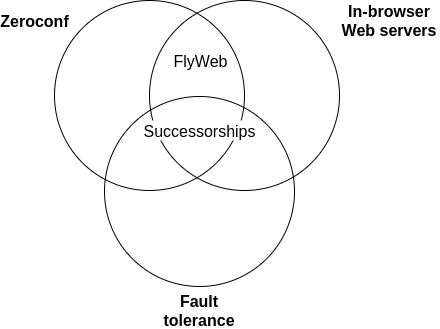
\includegraphics[keepaspectratio,width=6cm]{shippy-intersections}
      \label{fig:stack}
\end{figure}

\subsection{Zeroconf}
\label{sub:background_zeroconf}

Hosts connected to a network rely on maintaining a common consensus on such basic matters as addressing and name resolution, if they are to have any hope of communicating over that network.
This need is often fulfilled by specially-designated configuration servers, such as DHCP or DNS servers.
However, such servers can be absent in common networking situations, such as \textit{ad hoc} networks.
In such cases, it remains desirable for hosts to handle these matters in a seamless and cross-platform fashion, without the need for manual configuration.
This is the problem addressed by the group of protocols referred to as Zeroconf, short for ``Zero Configuration Networking''.\footnote{Although the term is sometimes used more broadly to designate any suite of technologies that seeks to address this problem, we observe the more specific meaning established by the former IETF Working Group by the same name.
See e.g. \url{http://www.zeroconf.org/}.}
Zeroconf protocols solve the problems of address allocation, address queries (mDNS), and network service discovery (DNS-SD), specifically when hosts share a direct link (be it logical or physical).
Since the first of these (address allocation) is a \textit{de facto} standard, as it has been integrated into consumer operating systems and printers since the early 2000s, we focus on the latter of these two here.

\textbf{Address queries.}
A name server can be used on a local network to maintain a mapping of logical names to IP addresses.
In the absence of such a server, a Zeroconf protocol called mDNS (short for ``multicast DNS'') can be used to formulate address queries on the local network.
As per its name, mDNS broadcasts these queries onto the local network rather than directing them to a single server; it also includes a mechanism to resolve naming conflicts~\cite{rfc6762}.
mDNS aims to handle any type of record lookup that could be handled by a DNS server, not just name-to-address lookups.
mDNS has grown steadily in popularity amongst networked devices; implementations of mDNS include Apple Bonjour, Spotify Connect, Philips Hue, Google Chromecast, and Avahi (an open-source implementation for Linux).

\textbf{Service discovery.}
Once connected to a network, a host may wish to learn about the services offered by the other devices connected to the network, such as printing or media streaming.
In a centrally-administered network, this may be accomplished by a directory server, such as a DNS server.
However, when such a server is lacking, the Zeroconf protocol called DNS-SD (``DNS service discovery'') leverages the ability to make distributed DNS queries provided by mDNS, to register, enumerate, and resolve local network services~\cite{rfc6763}.


\subsection{In-Browser Web Servers}
\label{sub:background_in_browser_web_servers}

More recently, a number of technologies have emerged to enable Web servers to be deployed entirely from within Web browsers.
Such technologies have the appeal that they simplify the process of serving Web content, thus potentially expanding the breadth of users capable of doing so.
For example, Opera Unite\footnote{\url{http://help.opera.com/Windows/12.10/en/unite.html}}, Web Server Chrome\footnote{\url{https://github.com/kzahel/web-server-chrome}}, PeerServer\footnote{\url{http://www.peer-server.com/}}, and FlyWeb\footnote{\url{http://flyweb.github.io/}} all enable browser applications to publish fully functioning Web servers.
We discuss FlyWeb below, and defer details on a few other approaches to Section \ref{sec:related_work}.

\subsection{The power of Zeroconf in the browser}
\label{sec:background_flyweb}

HTTP servers running on hosts that usually access the Web as clients face a few challenges not normally encountered by those running on dedicated server machines.
For example, they must be properly configured to circumvent firewalls, and they must ensure that other clients have a way of finding out their IP address.

The FlyWeb project, developed by the Mozilla Firefox community, addresses the problem of advertising and discovering in-browser Web services in the particular environment of local networks, by leveraging Zeroconf service advertisement and discovery.
To this end, FlyWeb provides two key pieces of functionality: 
\textit{(i)} an implementation of mDNS, allowing those services to advertise their name and address to peers on the local network, and 
\textit{(ii)} a FlyWeb service discovery menu, which uses a built-in implementation of DNS-SD to enumerate locally-discovered services.
The goal is for devices on a local network to be able to stream applications and content to one another using widely available Web technology.\footnote{\url{https://hacks.mozilla.org/2016/09/flyweb-pure-web-cross-device-interaction/}}
%FlyWeb was released in mid-2016, but is no longer actively maintained as of August 2017.

An important part of the appeal of this approach is its sheer versatility: it empowers any Web application with the ability to connect heterogeneous devices over an \textit{ad hoc} network, without each user needing to download a native app for their particular platform.
Examples of successful demonstrations of this idea include a collaborative photo sharing app, a printer interface, a temperature monitoring interface, and even a quadcopter controller.\footnote{\url{https://github.com/flyweb/examples}}


\subsection{The need for availability}
\label{sec:background_motivation}

A different challenge facing in-browser Web servers is that their availability is limited by that of the host machine.
Dedicated server machines usually have static network addresses and are often streamlined for serving Web content; however, the class of devices that can run a Web browser is much wider, including mobile devices, hence posing a novel challenge to service availability.
To the best of our knowledge, at the time of writing, none of the currently-existing technologies address the issue of recovering from disruptions of server availability for in-browser Web services.

We argue that application availability in the face of server failure is a requirement for many common use cases of client-server Web applications running on local networks.
This is especially true when one considers the current prevlance of networked mobile devices, where the server node might leave the local network, or fail due to other reasons such as low battery.

To motivate this concretely, consider a simple queuing Web application called \texttt{QueueApp}, which might be useful in the following scenario: a TA\footnote{Teaching Assistant} holds office hours in a small classroom, and students arrive at random intervals seeking individual assistance.
Students may arrive at a rate that exceeds that at which the TA is able to address their concerns, and so the TA wishes to keep track of the order in which they arrive.
The TA takes out her smartphone and loads \texttt{QueueApp}, which immediately starts a Web server on her phone.
As students arrive, she directs them to the URL of the local \texttt{QueueApp} service; when they connect, they are faced with an interface that enables them to either join the queue if they are not already in it, or to leave it if they are.
Now, say the TA needs to temporarily leave the room, for example to take an important phone call.
Unless special functionality is implemented by the application, the clients (students) will get disconnected from the server (TA), and the application state will need to be reset.

We argue that in such a case, it would be of great practical value for \texttt{QueueApp} to continue functioning seamlessly, even in the absence of the initial server.
What if 5 students enter the room while the TA is out?
In this paper, we make the case that those students should be able to enqueue despite the absence of the TA.

In the following section, we explain how we achieve this in the \APIName library.


\section{Proposed Approach}
\label{sec:approach}

Our goal is to build a framework to facilitate the development of offline client-server Web applications that robustly recover from server faults. 
We posit that the following features are prerequisites to achieving this:

\begin{enumerate}
    \item Any client, but exactly one client, has the ability to automatically assume the responsibilities of the server if the server goes down;
    \item All clients in the network have the capability to automatically update their connections to the new server in the event that the server migrates from one node to another;
    \item (Optional, if we have time) The initial server node has the ability to resume responsibilities of the server once it comes back online (and can be reasonably believed to be robustly online)
    
\end{enumerate}

The model we propose for achieving this is one in which clients connecting to the server automatically acquire distributed state including the following elements:

\begin{enumerate}
	\item Constant: A UUID for the initial host node (the first to serve the application);
    \item The current state of the server;
	\item A ``successorship'' list: a list of (potentially not all of the) nodes in the local network, in order of ``who is next'' to assume server responsibilities, in the event that the server goes down;
    \item Constant: The actual server code to execute, in the event that one of the clients needs to begin acting as the server.
\end{enumerate}

Note that the elements marked ``(Constant)'' are permanently fixed (for the lifetime of the application) when the initial server node first runs the application server.

We propose to develop a Javascript library that implements the functionality listed above, providing a clean interface to enable developers to seamlessly integrate fault-tolerance into their offline client-server Web applications, without having to worry about the details of how such fault-tolerance is achieved.

\subsection{API Overview}

Our current running name for the library is \texttt{\APIName}\footnote{We still need a proper acronym for it, e.g. \APIshort}, i.e. the next ship that will lead the flotilla after yet another sunk boat. We propose to implement the following interface in \APIName:


\begin{itemize}
	\item Server side:
    \begin{itemize}
    \begin{ttfamily}
      \item initServer(name)
      \item onReceive(msg, callback)
      \item commitState(callback)
    \end{ttfamily}
    \end{itemize}
    \item Client side:
    	\begin{itemize}
    	\begin{ttfamily}
    		\item initClient()
            \item connect(serverName)
            \item send(msg, payload)
    	\end{ttfamily}
    	\end{itemize}
\end{itemize}


We briefly discuss the major functions of our proposed API in the following subsections. Throughout the discussion, we use the TA queue example to illustrate our API usage.

{\bf Server initialization and service instantiation: } the first functions to initiate a server are {\ttfamily initServer} and {\ttfamily onReceive}. The former starts the local server in the device's browser and, after initialization, assigns a host name for that server. The later register entry points for services offered by that server.

In our queue system, one would initialize a server and define two functions to handle requests to enqueue students and also to dequeue them once they are helped. Additionally, the server provides the queue service in order to provide the current state of the queue. If no recognizable service is requested, the TAQueue server responds with the queue service.

\begin{lstlisting}[language=JavaScript]
    function getQueue(req, event) { ... }
    function handleEnqueue(req, event) { ... }
    function handleDequeue(req, event) { ... }

    (function main(){
        server = sship.initServer("TAQueue");
        server.onReceive('queue', getQueue, 
            default=true);
        server.onReceive('enqueue', handleEnqueue);
        server.onReceive('dequeue', handleDequeue);
    })();
\end{lstlisting}

{\bf Establishing connections: } as a server starts running, it broadcasts its name in the local-area network and clients in the same network can discover this server. A client device needs a single line of code to initialize itself. Upon initialization it will lookup for host servers in the network. Once a list of servers is retrieved and displayed, a client may select a server to connect to. In our TA queue example, we explicitly know the server name and skip the server list phase:

\begin{lstlisting}[language=JavaScript]
    (function main(){
        client = sship.initClient().connect("TAQueue");
    })();
\end{lstlisting}


{\bf Data exchange: } clients can ask for services through the {\ttfamily send} function. The function explicitly takes a requested service as one of its parameters and a payload as its second one. In our queue system, two distinct clients may request to enqueue themselves.

\begin{lstlisting}[language=JavaScript]
    (function main(){
        client1 = sship.initClient().connect("TAQueue");
        client1.send(enqueue, 
            {student: "Arthur", csid: "cs4321"});

        client2 = sship.initClient().connect("TAQueue");
        client2.send(enqueue, 
            {student: "Paul", csid: "cs9876"});
    })();
\end{lstlisting}

{\bf Updating the server state: } Finally, it is necessary to define which data structures or variables are important for a server, thus the {\ttfamily commitState} function receives a function which is executed every time that a service is successfully requested and executed in that server. Revisiting our {\ttfamily server = sship.initServer("TAQueue")} code snippet, we would add a final function to define how the server would be updated after queueing/dequeuing students.

\begin{lstlisting}[language=JavaScript]
    var queue = [];
    function currentQueue() { return queue; }

    (function main(){
        server = sship.initServer("TAQueue");
        ...
        server.commitState(currentQueue);
    })();
\end{lstlisting}


\subsection{Replication Strategy}

We aim to leverage the concepts of \textbf{eventual consistency} and \textbf{lazy replication} for our fault tolerance approach. 
We argue that our domain of local ad-hoc offline Web applications will mostly tolerate minor time frames of inconsistent states and we rather aim to increase availability and performance.

When a server is initialized and starts running, we envision that our API will create a state for that server and that this state is updated after the execution of any received message callback. 
As clients connect to a server, the clients themselves assign their own host names and the server keeps a list of connected clients.
Changes to the server state are broadcasted to all clients. 
A central concern, therefore, is to handle the possibility of inconsistencies in the versions of the server state maintained by each client: what if the server dies before changes are broadcasted? 
What if the broadcast to our next server fails and the next server takes over with a stale state? 

Our current idea is to converge to a consistent state in accordance with the eventual consistency principle when clients (re-)connect to the new server: upon connecting, they can send their current state associated with a timestamp of the last modification.
From this information, the most current version of the previous server's state can be determined from amongst all clients' copies, and then propagated to the new server.
This system opens up the risk of being spoofed by malicious clients imposing a manipulated state onto our network, but as stated previously, we allow ourselves to assume full trust between all participants in the network for simplification.
 
We have also considered using a CRDT for our implementation, but we believe that the constraint of commutativity of operations, or associativity of merging conflicting states, is potentially too restricting for the range of applications we would want to allow to run on our framework.


\subsection{Assumptions}

Our first version of this fault-tolerant extension to zero-configuration networks will necessarily have to make some simplifying assumptions, to make initial design and implementation tractable. 
In particular, we assume the following, fully realizing that these may not hold for real-world practical use cases:

\subsubsection*{The nodes in the network trust one another.} 

An implication of our model is that any node in the network (with a reliable connection) may at some point become the application server.
This status comes with all the responsibilities of the server, including executing the server-side application code, and hence maintaining the server-side application state.
Without any further substantial design considerations, this model would be extremely susceptible to a malicious client acquiring server status, and exploiting this status for their own ends, either by serving downright malicious material, or by more subtly forging application state.
For an example of the latter, consider once again the \texttt{queue} app; when the TA leaves the room and one of the student devices becomes the server, that student could leverage her trusted position as the new server by pushing herself to the front of the line.

\subsubsection*{Updates to server-side state are small.}

A core requirement of our model is that the server be able to broadcast its changes in state to all clients in the local network with relatively low latency, to diminish the possibility of clients' copies of server state being out of sync.
Therefore, we assume that communication in the network is not traffic intensive, i.e. nodes neither produce bursts of requests in a small period of time, nor do they have payloads higher than some threshold $\tau$ that might generate bottlenecks in the network.




\section{Evaluation}
\label{sec:evaluation}

\subsection{Sample Successorships Application}

In our previous project, we created a web application using the presentation framework \textit{Reveal.js}~\footnote{https://github.com/hakimel/reveal.js/, accessed 2019-04-17} to present Successorships to graduate students of the computer science department of the University of British Columbia.
The application used the Successorships API that made use of the Zeroconf protocols based on FlyWeb.
Obviously, the presenters had to have a Mac computer and a dedicated old version of Firefox Developer Edition with the FlyWeb addon installed to be able to present.
Moreover, the previously mentioned performance problems were clearly visible, with recovery of the system from intentionally injected faults taking over 20 seconds at times.
In a similar fashion, we presented Zeroties to an audience of graduate students at the same university.
The presentation technicalities remained the same, except that the API usage within Successorships was changed from FlyWeb to Zeroties.
To demonstrate this new independence of Firefox, the presentation was performed on Google Chrome.
A significant decrease in time-to-recovery after failure could clearly be observed with the system recovering in very few seconds.

\subsection{Empirical Evaluation}

We reproduced the performance measurements from the previous paper in order to analyze changes in performance from the old to the new version of Successorships.
We collected traces for system recovery for the following scenario, first with the old FlyWeb-based version on Mozilla Firefox, and then with the new Zeroties-based version on Google Chrome:
\begin{itemize}
\item One node starts the app and becomes the server.
\item 5 nodes start the app and become clients.
\item The server broadcasts 7 messages to all clients.
\item The server dies and the next successor becomes the server.
\item The other 4 clients become clients to the new server.
\end{itemize}

This process was first repeated until only the last node remained and became the server.
Afterwards, 5 more nodes started the application and became clients of that last remaining node from the last run that was now serving.
The process was then repeated once more until the last node was finally terminated.
In total, this process therefore involved 9 recoveries from server failures.
The scenario was performed on one machine where one node constituted one browser window.
While we acknowledge that a multi-machine experiment would have been more representative, we argue that for the analysis of performance changes between the two version this infrastructural change would not be significant.

Table~\ref{tbl:eval:time-to-recovery} shows the time to recovery in seconds for the described scenario with FlyWeb and Zeroties.
It is visible, that the Zeroties version recovered from failures nearly 10 times faster with little variation.
Figure~\ref{fig:eval:server-recovery} compares the cumulative distribution between the two versions that confirms this finding.

\begin{table}
    \caption{Time-to-recovery in seconds with FlyWeb and Zeroties}
    \label{tbl:eval:time-to-recovery}
    \centering
    \begin{small}
    \begin{tabular}{C{1cm}|C{2.5cm}|C{2.5cm}}
    \hline
    \bfseries Failure \# & \bfseries FlyWeb & \bfseries Zeroties \\
    \hline
1 & 15.554 & 1.817 \\
2 & 15.05 & 1.607 \\
3 & 13.183 & 1.701 \\
4 & 13.07 & 1.659 \\
5 & 14.836 & 1.795 \\
6 & 10.652 & 1.726 \\
7 & 11.32 & 1.244 \\
8 & 11.212 & 1.138 \\
9 & 11.473 & 1.269 \\
    \hline
    \end{tabular}
    \end{small}
\end{table}

\begin{figure}[h]
    \centering
    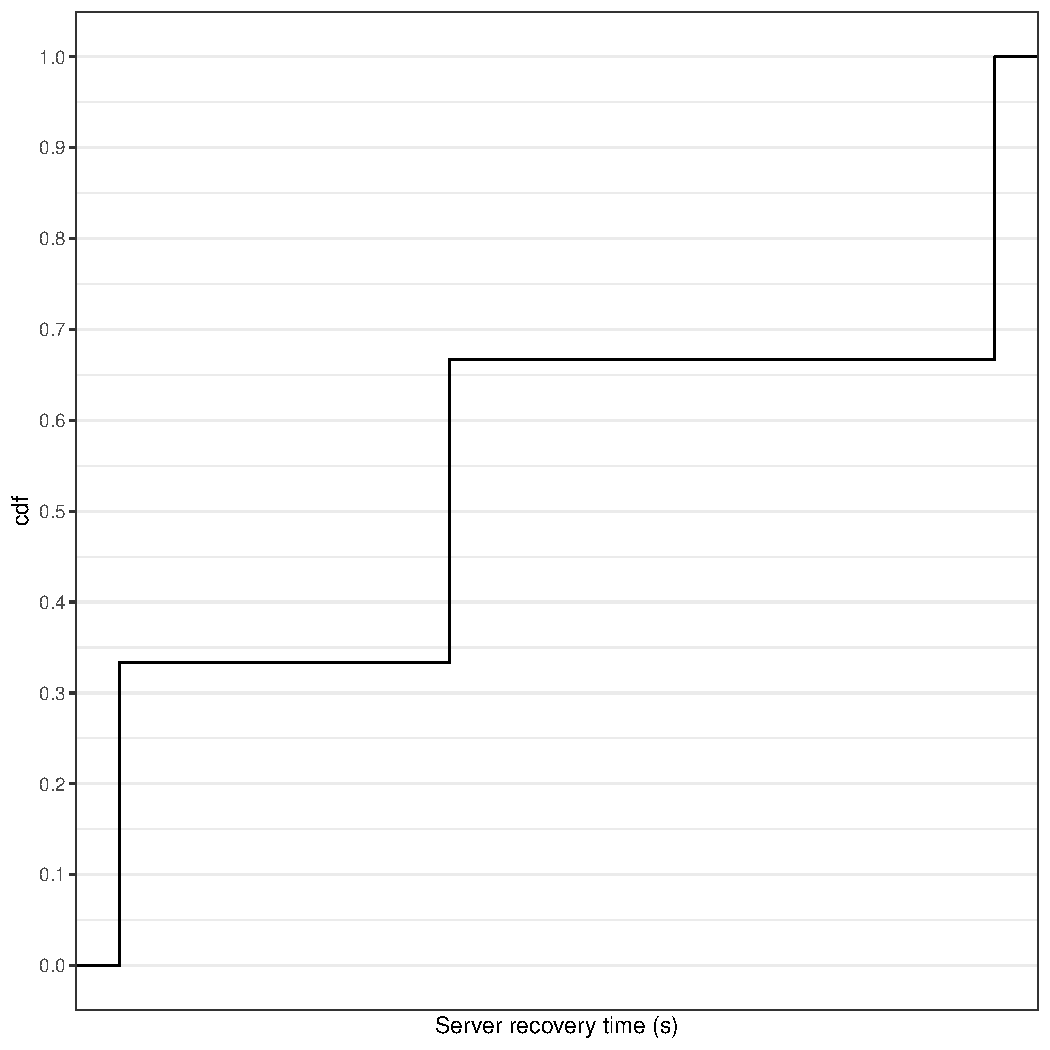
\includegraphics[keepaspectratio,width=\columnwidth]{server-recovery}
    \caption{Comparison of CDFs for server discovery between FlyWeb-based and Zeroties-based versions of Successorships.}
    \label{fig:eval:server-recovery}
\end{figure}

\section{Timeline}
\label{sec:timeline}

We consider late November as the project final deadline. With that in mind, there are a few key activities that we define as milestones, such that we keep up with the project schedule.

\begin{itemize}
    \item {\bf Oct 25th: } Study and evaluate replication patterns. Build a sample FlyWeb queue application;
    \item {\bf Nov 8st: } Implement the core functionalities of the \APIName{} API.
    \item {\bf Nov 15th: } Continue API implementation. Start writing scripts for evaluation;
    \item {\bf Nov 29nd: } Wrap-up API. Write scripts to analyze and plot data; Start drafting project report.
    \item {\bf Dec 11th: } Project deadline
\end{itemize}

\bibliographystyle{abbrv}
\bibliography{flyweb_paper}

\end{document}

